% Generated from preserved paired observations. Do not edit by hand.
\begin{figure}[htbp]
\centering
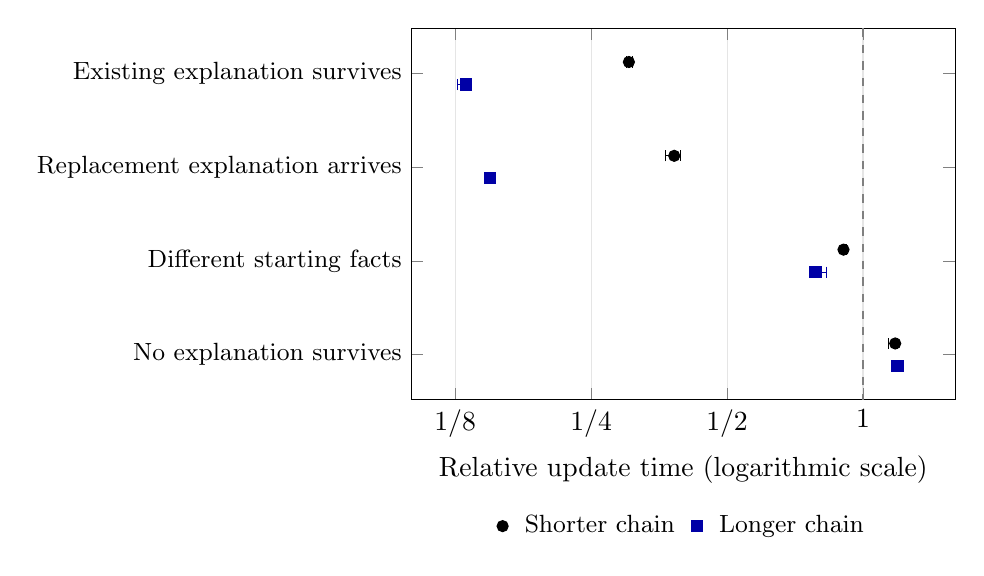
\begin{tikzpicture}
\begin{axis}[width=0.70\linewidth,height=6.3cm,xmode=log,
xmin=0.1,xmax=1.6,ymin=-0.48,ymax=3.48,y dir=reverse,
ytick={0,1,2,3},
yticklabels={{Existing explanation survives},{Replacement explanation arrives},{Different starting facts},{No explanation survives}},
yticklabel style={font=\small},
xlabel={Relative update time (logarithmic scale)},
xtick={0.125,0.25,0.5,1},xticklabels={1/8,1/4,1/2,1},
xmajorgrids=true,grid style={gray!20},
legend style={at={(0.5,-0.28)},anchor=north,draw=none,font=\small,column sep=4pt},
legend columns=2]
\addplot[gray,dashed,forget plot] coordinates {(1,-0.48) (1,3.48)};
\addplot[only marks,mark=*,black,error bars/.cd,x dir=both,x explicit]
coordinates {
(0.303107186,-0.12) += (0.005380192,0) -= (0.003875500,0)
(0.381928514,0.88) += (0.012880738,0) -= (0.016163149,0)
(0.905277511,1.88) += (0.011728574,0) -= (0.005298335,0)
(1.178358201,2.88) += (0.016322907,0) -= (0.041958422,0)
};
\addlegendentry{Shorter chain}
\addplot[only marks,mark=square*,blue!65!black,error bars/.cd,x dir=both,x explicit]
coordinates {
(0.132315292,0.12) += (0.001499708,0) -= (0.005665689,0)
(0.149473165,1.12) += (0.003692939,0) -= (0.001777688,0)
(0.784898536,2.12) += (0.047034643,0) -= (0.012522867,0)
(1.187932124,3.12) += (0.040023678,0) -= (0.034218154,0)
};
\addlegendentry{Longer chain}
\end{axis}
\end{tikzpicture}
\caption{Sharing explanations reduces the cost of updating knowledge when conclusions remain justified, but adds work when their justification disappears. The experiment changes facts and rules in cyclic chains concerning 256 individuals; the shorter and longer chains have four and 32 links before the cycle closes. Points show median time with shared explanations divided by ordinary maintenance time, from nine paired repetitions per case in an independent replication. Bars show descriptive 95\% paired bootstrap intervals (2,000 resamples). Values left of the dashed line indicate faster updating.}
\label{fig:scientific-support}
\end{figure}

\begin{table}[htbp]
\centering\small
\caption{The principal comparisons answer different scientific questions; they do not establish an overall ranking of reasoning systems. Performance changes are derived from median paired time ratios on the same machine. Query timings in the fourth row exclude data preparation.}
\label{tab:scientific-evidence}
\begin{tabularx}{\linewidth}{@{}>{\raggedright\arraybackslash}p{0.19\linewidth}>{\raggedright\arraybackslash}X>{\raggedright\arraybackslash}X@{}}
\toprule
Evidence & Comparison & Principal finding \\
\midrule
University ontology & Full LUBM ontology and its 14 standard questions. & All reference answers recovered in every repetition. \\[4pt]
Changes to rules & Established university rule program, compared with the reference version. & Rule additions 2.1--3.2\,$\times$ faster; removals 1.4--1.6\,$\times$ faster. \\[4pt]
External rule reasoner & The same rule changes, compared with ZodiacEdge. & One addition 6.2\,$\times$ faster; one removal 41\,$\times$ slower. \\[4pt]
Order of reasoning & A difficult TPC-H Q5 component and four deliberately adverse controls. & Q5 needs 49\% less query time; controls need 7--24\% more. \\[4pt]
Broader OWL reasoner & Selected DLP L3 task, compared with HermiT at three data sizes. & 2.6--21.5\,$\times$ faster; the tested family also belongs to OWL 2 EL. \\[4pt]
\bottomrule
\end{tabularx}
\end{table}
